\documentclass{article}
\PassOptionsToPackage{sort,numbers,square}{natbib}

\usepackage{nips_2018}
\usepackage[utf8]{inputenc} % allow utf-8 input
\usepackage[T1]{fontenc}    % use 8-bit T1 fonts
\usepackage{hyperref}       % hyperlinks
\usepackage{url}            % simple URL typesetting
\usepackage{booktabs}       % professional-quality tables
\usepackage{amsfonts}       % blackboard math symbols
\usepackage{nicefrac}       % compact symbols for 1/2, etc.
\usepackage{microtype}      % microtypography

% For citations
\usepackage{natbib}

% For algorithms
\usepackage{algorithm}
\usepackage{algorithmic}
\usepackage{hyperref}
\hypersetup{backref,colorlinks=true,citecolor=blue,linkcolor=blue,urlcolor=blue}

%\newcommand{\theHalgorithm}{\arabic{algorithm}}


\usepackage{graphicx}
\usepackage{subfigure} 
\graphicspath{{../nips-2018/}}


%Arash
\usepackage{amsmath,amsthm}
\usepackage{amssymb}
\usepackage{mathrsfs}
\DeclareMathOperator*{\argmin}{argmin}
\usepackage{siunitx}
\usepackage{comment}
\usepackage{mathtools}
\mathtoolsset{showonlyrefs}

\renewcommand*{\figureautorefname}{Figure}%
\renewcommand*{\tableautorefname}{Table}%
\renewcommand*{\sectionautorefname}{Section}%
\renewcommand*{\subsectionautorefname}{Section}%
\renewcommand*{\subsubsectionautorefname}{Section}%

\newtheorem{theorem}{Theorem}%[section]
\newtheorem{definition}[theorem]{Definition}
\newtheorem{lemma}[theorem]{Lemma}



\usepackage{gensymb}
\usepackage{xcolor}
\newcommand{\attn}[1]{\textcolor{red}{TODO: #1}}
\newcommand{\one}{\mathbf{1}}
\renewcommand{\algorithmiccomment}[1]{\hfill $\rhd$ #1}
\newcommand{\given}{\;\vert\;}
\newcommand*{\algorithmautorefname}{Algorithm}%
\newcommand{\norm}[1]{\left\lVert #1 \right\rVert}
\DeclareMathOperator*{\prox}{\bf prox}
\DeclareMathOperator*{\sign}{sign}

\usepackage{xr}
\externaldocument{paper-supplement}




\title{Modeling trend in temperature volatility using generalized LASSO}

\author{Arash Khodadadi\\
 Department of Statistics\\
 Indiana University\\
 Bloomington, IN 47408 \\
 \texttt{arakhoda@indiana.edu}
\And
  Daniel J.\ McDonald \\
 Department of Statistics\\
 Indiana University\\
 Bloomington, IN 47408 \\
 \texttt{dajmcdon@indiana.edu}}


\begin{document} 


\maketitle


\begin{abstract}
In this paper, we present methodology for estimating trends in
spatio-temporal volatility. We give two algorithms for computing our
estimator which are tailored for dense, gridded observations over both
space and time, though these can be easily extended to other
structures (time-varying network flows, neuroimaging). We motivate our
methodology by applying it to a massive climate dataset and
discuss the implications for climate analysis.
\end{abstract}



\section{Introduction}

Estimating smooth trends over time for large collections of time
series is a common problem in economics, finance, meteorology,
neuroscience and more. Most of this work focuses on analyzing trends
(or removing trends) in the temporal average, but trends in variance
can be more relevant, especially for financial data but also for
climate science.

Trends in terrestrial temperature variability are perhaps more relavant for species
viability than trends in mean
temperature~\citep{huntingford_no_2013},
because, an increase in the
temperature variability will increase the probability of extreme hot
outliers~\citep{VasseurDeLong2014}. Recent climate literature
suggests that it is more difficult for society to adapt to these
extremes than to the gradual increase in the mean temperature
\citep{hansen_perception_2012,huntingford_no_2013}. Furthermore, the willingness of popular media to
emphasize the prevalence extreme cold events coupled with a
fundamental misunderstanding of the relationship between climate (the global
distribution of weather over the long run) and weather (observed
short-term, localized behavior) leads to public misunderstanding of climate
change. In fact, increased frequency of extreme cold events in the
northern hemisphere can be partially attributed to increases in
mean climate but is also due to increases in temperature
variance~\citep{Screen2014,FischerBeyerle2013,TrenberthZhang2014}. 

Nevertheless, research examining trends in the volatility of
spatio-temporal climate data is scarce. \citep{hansen_perception_2012} studied the change in
the standard deviation (SD) of the surface temperature in the NASA
Goddard Institute for Space Studies gridded temperature data set by
examining the empirical SD at each spatial location relative to that
location's SD over a base period, and showed
that these estimates are increasing.
\citep{huntingford_no_2013} took a similar
approach in analyzing the ERA-40 data set. Their results showed that there
still is an increase in the SDs from 1958-1970 to 1991-2001, but this
is much less than what is obtained from the method used in
\citep{hansen_perception_2012}. The authors also computed the
time-evolving global SD from the de-trended time-series at each
position, which suggests that the global SD has been
stable. 

These and other related research, e.g.,
\citep{rhines_frequent_2013}, have several shortcomings. First, no
statistical analysis has been performed to examine if the changes in
the SD are statistically significant. Second, the methodologies for
computing the SDs are highly sensitive to the choice of base period. Third,
and most importantly, temporal and spatial correlations between the
observations are ignored.  


\subsection{Related work}

Variance estimation for financial time series has a lengthy history,
focused especially on parametric models like the generalized
autoregressive conditional heteroskedasticity (GARCH) process~\citep{engle2002dynamic} and
stochastic volatility models~\citep{HarveyRuiz1994}. These models (and
related AR processes) are specifically for parametric modelling of
short ``bursts'' of high volatility, behavior typical of financial
instruments. Parametric models for spatial data go back at least
to~\citep{besag1974spatial} who proposed a conditional probability
model on the lattice for examining plant ecology.

More recently, nonparametric models for both spatial and temporal data
have focused on using $\ell_1$-regularization for trend
estimation. \citep{KimKoh2009} proposed $\ell_1$-trend filtering for
univariate time series, which forms the basis of our methods. These
methods have been generalized to higher order temporal smoothness
~\citep{Tibshirani2014}, graph dependencies~\citep{WangSharpnack2016},
and, most recently, small, time-varying
graphs~\citep{HallacPark2017}. Our methodology is similar in flavor
to~\citep{HallacPark2017}, though it uses a different likelihood
function to emphasize variance estimation rather than trends in mean
signal. Furthermore, the focus is in high-dimensional, regular data
rather than a small number of changing graphs.

\subsection{Main contributions}

The main contribution of this work is to develop a new methodology for
detecting the trend in the volatility of spatio-temporal data. In this
methodology, the variance at each position and time is considered as
a hidden variable. The values of these hidden variables
are then estimated by maximizing the likelihood of the observed
data. We show that this formulation is not appropriate for
detecting the trend, so, following ~\citep{Tibshirani2014}, we penalize the
differences between the estimated variances which
are temporally and spatially ``close'', resulting
in a generalized LASSO problem. % However, the
% dimension of this optimization problem is very high and so the
% standard methods solvers are inadequate. We develop two algorithms
% which are computationally feasible. In the first method, we adopt an optimization technique
% called alternative direction method of multipliers (ADMM)
% \citep{boyd_distributed_2011}, to divide the total problem into
% several sub-problems of much lower dimension and show how the total
% problem can be solved by iteratively solving these sub-problems. The
% second method, called the \textit{linearized ADMM algorithm}
% \citep{parikh_proximal_2014} solves the main problem by iteratively
% solving a linearized version of it. We will compare the benefits of
% each method. 

Our main contributions are as follows:
\begin{enumerate}
\item We propose a model for nonparametric variance estimation for a
  spatio-temporal process (\autoref{sec:ell_1-trend-filt}).
\item We derive two alternating direction method of multiplier
  algorithms (ADMM) to fit our estimator when applied to 
  very large data (\autoref{sec:prop-optim-meth}). We give situations
  under which each algorithm is most likely to be useful.
\item We illustrate our methods on a large global temperature dataset
  with the goal of tracking world-wide trends in variance as well as a
  simulation constructed to mimic these data's features
  (\autoref{sec:empirical-evaluation}). 
\end{enumerate}

While we motivate and illustrate our methods on large, gridded climate
data, we note that our algorithms are also applicable to neuroimaging
data or large collections of financial instruments.

\section{Estimating the variance of spatio-temporal data}
\label{sec:ell_1-trend-filt}


$\ell_1$-trend filtering was proposed by \citep{KimKoh2009} as a
method for estimating a smooth, time-varying trend. It is formulated
as the optimization problem 
% : a time-series $y_t$, $t=1,...,T$ is observed and we believe that
% it consists of a smooth trend and a stochastic component and the
% goal is to estimate the trend. The estimated trend is desired to be
% smooth, but at the same time, we seek small estimated residuals
% (stochastic component). These two objectives cannot be achieved
% simultaneously and so a trade-off between them should be made. In
% $\ell_1$-trend filtering, this trade-off is formulated as the
% following convex optimization problem: 
$
\min_{\beta} \frac{1}{2} \sum_{t=1}^{T} (y_t-\beta_t)^2+\lambda
\sum_{t=1}^{T-2} \left|\beta_t-2\beta_{t+1}+\beta_{t+2}\right| 
$
or equivalently:
\begin{equation}
\min_{\beta} \frac{1}{2} \norm{ y-\beta }_2^2+\lambda \norm{ D\beta}_1
\label{eq:l1tf}
\end{equation}
 where $y_t$ is an observed time-series, $\beta$ is the smooth trend,
 $D$ is a $(T-2)\times T$ matrix, and $\lambda$ is a tuning parameter
 which balances fidelity to the data (small errors in the first term)
 with a desire for smoothness.  
% The \textit{penalty matrix} is:
% \begin{equation}
% D=\begin{bmatrix}
% 1 & -2 & 1 &  &  &  &\\ 
% & 1 & -2 & 1 &  &  &\\ 
% &  & \ddots & \ddots & \ddots  &  &\\ 
% &  & & 1 & -2 & 1 &  \\ 
% &  &  &   & 1 & -2 & 1 
% \end{bmatrix}
% \label{eq:d_matrix}
% \end{equation}
%The first term in \eqref{eq:l1tf} penalizes large residuals while the second term encourages smooth estimated $\beta$.
With the penalty matrix $D$, the estimated $\beta$ will be piecewise
linear. \citep{KimKoh2009} proposed a specialized primal-dual
interior point (PDIP) algorithm for solving \eqref{eq:l1tf}. From a
statistical perspective, \eqref{eq:l1tf} is a constrained maximum
likelihood problem with independent observations from a normal
distribution with common variance, $y_t \sim \mbox{N}(\beta_t,
\sigma^2)$, subject to a piecewise linear constraint on $\beta$. 

% The results of applying $\ell_1$-trend filtering on the Bloomington
% time-series are shown in \autoref{fig:bloom_detrended}. The left
% panel shows the original time-series (blue) together with the
% estimated $\beta$ (red) and the right panel shows the residuals
% $y_t-\beta_t$ (blue). As it can be seen, the estimated $\beta$s are
% piecewise linear. The number of linear segments is determined by the
% value of $\lambda$. Here, we chose $\lambda=500$. The choice of
% $\lambda$ is a model selection problem and we will return to it in
% the next section ???. 

\subsection{Estimating the variance}
\label{sec:l1tf_var}


Inspired by the $\ell_1$-trend filtering algorithm, we propose a
non-parametric model for estimating the variance of a time-series. To
this end, we assume that at each time step $t$, there is a hidden
variable $h_t$ such that conditioned on $h_t$ the observations $y_t$
are independent normal variables with zero mean and variance
$\exp(h_t)$. The negative log-likelihood of the observed data in this
model is $l(y\given h) \propto -\sum_{t=1}^T h_t - y_t^2e^{-h_t}$. Crucially,
we assume that the hidden variables $h_t$ vary smoothly. To impose
this assumption, we estimate $h_t$ by solving the penalized, negative
log-likelihood: 
\begin{equation}
\min_h -l(y\given h)+\lambda \norm{ Dh }_1
\label{eq:l1tf_var}
\end{equation}
 where $D$ has the same structure as above.

As with~\eqref{eq:l1tf}, one can solve~\eqref{eq:l1tf_var} using the
PDIP algorithm (as in, e.g.,
\texttt{cvxopt}~\citep{andersen_cvxopt:_2013}). In each iteration of
PDIP we need to compute a search direction by taking a Newton
step on a system of nonlinear equations. Due to space limitations, we
defer details to Appendix A in the Supplement, where we show how to derive the dual of this optimization problem and compute the first and second derivatives of the dual objective function. 


\begin{comment}
\begin{algorithm}[tb]
  \caption{PDIP for $\ell_1$ variance estimation}
  \label{alg:pdip}
  \begin{algorithmic}
    \REQUIRE $\lambda>0$, $w>0$, $\nu\leftarrow 0$, $\mu_1\leftarrow
    0$, $\mu_2\leftarrow 0$, $J\in\mathbb{Z}^+$, $\{w_k\}$
    \COMMENT{Initialization} 
    \FOR[Central path]{$k=1,2,\ldots$}
    \FOR[Newton updates]{$j=1,\ldots,J$}
    \STATE Solve $A [\Delta\nu\; \Delta\mu_1\;
    \Delta\mu_2]^\top=r_{w_k}$ to find the search direction. 
    \STATE $\quad\quad A$ is given in \ref{eq:delta_r}
    \STATE Update $[\nu^{j+1}\; \mu^{j+1}_1\; \mu^{j+1}_2] \leftarrow
    [\nu^{j}\; \mu^{j}_1\; \mu^{j}_2] + [\Delta\nu\; \Delta\mu_1\;
    \Delta\mu_2]$. 
    \ENDFOR
   \ENDFOR
   \RETURN $h=\log\frac{y^2}{1+D^\top\nu}$ 
   \\
   \attn{Is this right? Explicit form of $A$}\\
   \attn{Arash: see appendix A}
  \end{algorithmic}
\end{algorithm}
\end{comment}

\subsection{Adding spatial constraints}
\label{sec:exten}

The method in the previous section can be used to estimate the
variance of a single time-series. In this section, we extend this
method to the estimation of the variance of spatio-temporal data. 

At a specific time $t$, the data is measured on a grid of points with
$n_r$ rows and $n_c$ columns for a total of $S=n_r\times n_c$ spatial
locations. Let $y_{ijt}$ denote the value of the 
observation at time $t$ on the $i^\text{th}$ row and $j^\text{th}$
column of the grid, and $h_{ijt}$ denote the corresponding hidden
variable. We seek to impose both temporal and spatial smoothness
constraints on the hidden variables. Specifically, we seek a solution
for $h$ which is piecewise linear in time and piecewise constant in
space (although higher-order smoothness can be imposed with minimal
alterations to the methodology). We achieve this goal
by solving the following optimization problem: 
\begin{align}
\min_h &\sum_{i,j,t}h_{ijt}+y_{ijt}^2e^{-h_{ijt}}
+\lambda_1 \sum_{i,j} \sum_{t=1}^{T-2} \left|h_{ijt}-2h_{ij(t+1)}+h_{ij(t+2)}\right|\\
&\quad+\lambda_2 \sum_{t,j} \sum_{i=1}^{n_r-1} \left|h_{ijt}-h_{(i+1)jt}\right|
+\lambda_2 \sum_{t,i} \sum_{j=1}^{n_c-1} \left|h_{ijt}-h_{i(j+1)t}\right|
\label{eq:l1tf_var_st}.
\end{align}

The first term in the objective is proportional to the negative
log-likelihood, the second is the temporal penalty for the
time-series at each location $(i,j)$, while the third and fourth,
penalize the difference between the estimated variance of two
vertically and horizontally adjacent points, respectively. The spatial
component of this
penalty is a special case of trend filtering on graphs~\citep{WangSharpnack2016} which penalizes the difference between the estimated values of the signal on the connected nodes. As before, we can write \eqref{eq:l1tf_var_st} in matrix form where $h$ is an $T\times S$ vector and $D$ is replaced by $D_{ST} \in \mathbb{R}^{(N_t+N_s) \times (T \cdot S)	}$, where $N_t=S \cdot (T-2)$ and $N_s=T \cdot (2n_rn_c-n_r)$ are the number of temporal and spatial constraints, respectively\footnote{$N_s$ is obtained by counting the number of unique constraints at each location and at all times.}. The exact form of this matrix in clarified in Appendix A in the Supplement. Then, as we have two different tuning parameters for the temporal and spatial components, we write $\Lambda =\left[\lambda_1\one_{N_t}^\top,\;  \lambda_2\one_{N_s}^\top\right]^\top$ leading to:\footnote{Throughout the paper, we use $|x|$ for both scalars and vectors. For vectors we use this to denote a vector obtained by taking the absolute value of each entry of $x$.} 
% let $h$ be a
% vector whose first $T$ entries are $h_{11t}$ for $t=1,...,T$, its next
% $T$ entries are $h_{21t}$ and so on, then the optimization problem in
% the matrix form is as
\begin{equation}
\min_h -l(y\given h)+ \Lambda^\top | D_{ST}h |.
\label{eq:l1tf_var_st_mat}
\end{equation}

\section{Proposed optimization methods}
\label{sec:prop-optim-meth}

For a spatial grid of size $S$ and $T$ time steps, $D_{ST}$ will have
$3Tn_rn_c-2n_rn_c-Tn_r$ rows and $ST$ columns. For a $1^\circ\times
1^\circ$ grid over the entire northern hemisphere and daily data over
10 years, we have $n_r=90$, $n_c=360$, $T=3650$ and so $D_{ST}$ has
approximately $10^8$ columns and $10^8$ rows. In each step of the PDIP
algorithm, we need to solve a linear system of equations which
depends on $D_{ST}^\top D_{ST}$ (see appendix A and B). Therefore,
applying the PDIP directly is infeasible for our data.\footnote{We
  note that this is a highly structured and sparse matrix, but, unlike
  trend filtering alone, it is not banded. We are unaware of general
  linear algebra techniques for inverting such matrix, despite our
  best efforts.}  

In the next section, we develop two ADMM algorithms for solving this
problem efficiently. The first casts the problem as a
so-called consensus optimization problem~\citep{boyd_distributed_2011}
which solves smaller sub-problems using PDIP and then recombines the results. The
second uses proximal methods to avoid matrix inversions.
 

\subsection{Consensus optimization}
\label{sec:consOpt}

\begin{comment}
General (unconstrained) optimization problems $\min_z
\sum_i f_i(z)$, $z\in\mathbb{R}^n$ can be rewritten equivalently using a
collection of local variables, $x_i\in \mathbb{R}^{n_i}$, and a
constraint. Following the notation of 
\citep{boyd_distributed_2011}, let $k=\mathscr{G}(i,j)$ which
means that the $j^\text{th}$ entry of $x_i$ is $z_k$ (or
$(x_i)_j=z_k$) and define $\tilde{z}_i \in \mathbb{R}^{n_i}$ by
$(\tilde{z}_i)_j=(x_i)_j$. Then the original unconstrained
optimization problem is equivalent to the following constrained
problem
$\min_{\{x_1,...,x_N  \}} \sum_i f_i(x_i)$ subject to $\tilde{z}_i=x_i$.
Now, we can apply ADMM to the augmented Lagrangian of this
problem: 
\begin{align}
x_i&\leftarrow \argmin_{x_i} f_i(x_i) + (u_i)^\top x_i +
     (\rho/2) \norm{ x_i-\tilde{z}_i }_2^2\\
%\label{eq:ADMM_steps}
z_k&\leftarrow (1/S_k)\sum_{\mathscr{G}(i,j)=k} (x_i)_j\\
u_i&\leftarrow u_i + \rho (x_i-\tilde{z}_i)
\end{align}
\end{comment}

Consider an optimization problem of the form $\min_h f(h)$, where
$h\in\mathbb{R}^n$ is the \textit{global variable} and
$f(h):\mathbb{R}^n \rightarrow \mathbb{R}\cup \{+\infty\}$ is
convex. Consensus optimization breaks this problem
into several smaller sub-problems that can be solved independently in
each iteration of optimization.  

Assume it is possible to define a set of local variables
$x_i \in \mathbb{R}^{n_i}$ such that $f(h)=\sum_i f_i(x_i)$, where
each $x_i$ is a subset of the global variable $h$. More specifically,
each entry of the local variables corresponds to an entry of the
global variable. Therefore we can define a mapping $\mathscr{G}(i,j)$
from the local variable indices into the global variable indices:
$k=\mathscr{G}(i,j)$ means that the $j^\text{th}$ entry of $x_i$ is
$h_k$ (or $(x_i)_j=h_k$). For ease of notation, define $\tilde{h}_i
\in \mathbb{R}^{n_i}$ as $(\tilde{h}_i)_j=h_{\mathscr{G}(i,j)}$. Then,
the original optimization problem is equivalent to the following
problem:  
\begin{equation}
\begin{aligned}
\min_{\{x_1,...,x_N  \}} \sum_i f_i(x_i)\\
 s.t. \,\,\, \tilde{h}_i=x_i. \,\,\,\,\,\,
\end{aligned}
\label{eq:consADMM}
\end{equation}
It is important to note that each entry of the global variable may
correspond to several entries of the local variables and so the
constraints $\tilde{h}_i=x_i$ enforce the consensus between the local
variables corresponding to the same global variable.  
The \textit{augmented Lagrangian} corresponding to 
\eqref{eq:consADMM} is $L_\rho(x,h,y)=\sum_i
\big(f_i(x_i)+u_i^\top(x_i-\tilde{h}_i) + (\rho/2) \lVert
x_i-\tilde{h}_i \lVert_2^2 \big)$. Now, we can apply ADMM to $L_\rho$. This results in solving $N$ independent optimization problems followed by a step to achieve consensus among the solutions in each iteration.
% which results in the following ADMM updates:
% \begin{align}
% x_i&\leftarrow\argmin_{x_i} f_i(x_i) + (u_i)^\top x_i +
%      (\rho/2)  \norm{ x_i-\tilde{h}_i }_2^2\\
% h_k&\leftarrow (1/S_k)\sum_{\mathscr{G}(i,j)=k} (x_i)_j \label{eq:ADMM_steps}\\
% u_i&\leftarrow u_i + \rho (x_i-\tilde{h}_i).
% \end{align}
% \attn{If you hate the left arrow, that's fine. But change it
%   everywhere, and use $=$. The $:=$ notation means that ``thing on
%   left is defined to be thing on right'' and isn't really appropriate here.}
% Here, $S_k$ is the number of local variable entries that correspond to
% $h_k$, and $u_i$ are the Lagrange multipliers.  
To solve the optimization problem \eqref{eq:l1tf_var_st_mat} using
this method, we need to address two 
questions: first, how to choose the 
local variables $x_i$, and second, how to the update them.
\begin{figure}[tb]
  \centering
  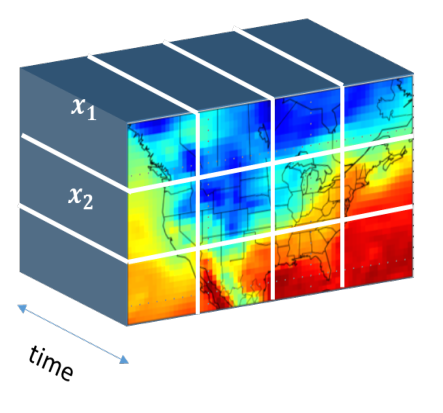
\includegraphics[height=.13\textheight]{Figures/data_cube}
  \caption{The cube represents the global variable $h$ in space and
    time. The sub-cubes specified by the white lines are
    $x_i$.}
  \label{fig:data_cube}
\end{figure} 


In \autoref{fig:data_cube}, the global variable $h$ is represented
as a cube. We decompose $h$
into sub-cubes as shown by white lines. Each local variable inside the sub-cubes corresponds to only one global variable. The local variables on the border (white lines), however, correspond to more than one global variable. With
this definition of $x_i$, the objective
\eqref{eq:l1tf_var_st_mat} decomposes as $\sum_i f_i(x_i)$ where
$f_i(x_i)=-l(y_i\given x_i)+\Lambda_{(i)}^\top |D_{(i)}x_i|$, and
$\Lambda_{(i)}$ and $D_{(i)}$ contain the temporal and spatial
penalties corresponding to $x_i$ only in one sub-cube. Thus, we now need to use PDIP to solve $N$ problems each of size $n_i$, which is feasible for small enough $n_i$. \autoref{alg:conADMM} gives the general version of this algorithm. A more detailed discussion of this is in Appendix B of the Supplement where we show how to compute the dual and the derivatives of the augmented Lagrangian. 

\begin{algorithm}[tb]
  \caption{Consensus ADMM }
  \label{alg:conADMM}
  \begin{algorithmic}
    \STATE {\bfseries Input:} data $y$, penalty matrix $D$, 
    $\epsilon, \rho,\lambda_t,\lambda_s >0$.
    \STATE {\bf Set:} $h\leftarrow 0$, $z\leftarrow 0$, $u\leftarrow
    0$. \COMMENT{Initialization} 
    \REPEAT
    \STATE $x_i\leftarrow\argmin_{x_i} -l(y_i\given
    x_i)+\Lambda_{(i)}^\top |D_{(i)}x_i|$
    \STATE $\quad\quad\quad+ (u_i)^\top x_i +
    (\rho/2)  \lVert x_i-\tilde{h}_i \rVert_2^2$. \COMMENT{Update local
      vars using PDIP}
    \STATE $h_k\leftarrow (1/S_k)\sum_{\mathscr{G}(i,j)=k} (x_i)_j
    $. \COMMENT{Global update.}
    \STATE $ u_i\leftarrow u_i + \rho (x_i-\tilde{h}_i)$. \COMMENT{Dual update}
    \UNTIL {$\norm{h^{m+1}-h^m}_2^2\ < \epsilon$}
    \STATE {\bf Return:} $h$.
  \end{algorithmic}
\end{algorithm}



Because consensus ADMM breaks the large optimization into
sub-problems that can be solved independently, it is amenable to a
split-gather parallelization strategy via, e.g., the map reduce framework.
In each iteration, the
computation time will be equal to the time to solve each sub-problem
plus the time to communicate the solutions on the master processor
and perform the consensus step. Since each sub-problem is
small, with parallelization, the computation time in each iteration
will be small. In addition, our experiments with several values of
$\lambda_t$ and $\lambda_s$ showed that the algorithm converges in few
hundreds iterations. 
% \attn{Need to redo this:}Solving each sub-problem on a machine with four
% 3.20GHz Intel i5-3470 cores takes less than 3 seconds on average, and
% so for example if we assume that communication time is 10 seconds and
% the algorithm converges in 300 iterations, with parallelization on
% $N_{sub-cubes}$ machines, the algorithm will converge in about 1
% hour. Assuming that we use $N_{sub-cubes}$ machines and that the
% convergence rate of the algorithm is independent of the grid size,
% this time will be independent of the grid size. 
% If we perform these computations on a single machine, the computation
% time grows linearly with $N_{sub-cubes}$. For example, for the data in
% a grid over the united states and using $3\times3\times521$ sub-cubes
% each iteration of the algorithm will take about 20 minutes on a single
% machine and so with 300 iterations it will take several days to
% converge. Given that we need to compute the solution for several
% values of the parameters $\lambda_t$ and $\lambda_s$, this computation
% time is not feasible. 
However, this algorithm is only useful if we can parallelize the
computation over several machines. In the next section, we describe
another algorithm which makes the computation feasible on a single
machine. 

\subsection{Linearized ADMM}
\label{sec:linADMM}

% In this section, we describe \textit{Linearized ADMM algorithm} \citep{parikh_proximal_2014} which, as we will see, makes the computation on a single machine feasible.

Consider the generic optimization problem
$\min_x f(x)+g(Dx)$
where $x\in \mathbb{R}^n$ and $D\in \mathbb{R}^{m\times n}$. Each
iteration of the linearized ADMM
algorithm~\citep{parikh_proximal_2014} for solving this problem 
has the form
\begin{align}
x & \leftarrow \prox_{\mu f} \left(x - (\mu/\rho)D^\top (D x - z + u )\right)\\
z & \leftarrow \prox_{\rho g} \left(z + u\right) \label{eq:linADMM_steps}\\
u & \leftarrow u + D x - z
\end{align}
where the algorithm parameters $\mu$ and $\rho$ satisfy $0 < \mu < \rho/\norm{D}_2^2$, $z,u\in \mathbb{R}^m$ and the proximal operator is defined as $\prox_{\alpha f}(u) = \min_x \,\, \alpha \cdot f(x)+\frac{1}{2} \norm{ x-u}_2^2$. Proximal algorithms are feasible when these proximal operators can be evaluated efficiently which, as we show next, is the case for our problem. 

%Clearly, \eqref{eq:l1tf_var_st} has this form necessary for using this algorithm.
% The optimization problem 
% form \eqref{eq:linADMM_opt} by defining
% \begin{align}
% & f(x):= \sum_{k} f_k(x_k) := \sum_{k}x_k+y_{k}^2e^{-x_{k}}\\
% & g(z):= \sum_{l} g_l(z_l) := \sum_{l} \lambda_l |z_l|\label{eq:linADMM_fg}\\
% & z = Dx
% \end{align}
% where $y_k$ is the $k^{th}$ entry of the vector whose entries are
% $y_{ijt}$, and $\lambda_l$ is the $l^{th}$ entry of the vector
% $\Lambda^\top=(\lambda_t\textbf{e}_{n_t}^\top|\lambda_s\textbf{e}_{n_s}^\top)$
% (see \autoref{sec:exten}). 
% To perform the steps in \eqref{eq:linADMM_steps}, we need to evaluate
% $\prox_{\mu f}$ and $\prox_{\rho g}$. 
 


\begin{lemma}
  Let $f(h) = \sum_{k} h_{k} + y_{k}^2e^{-h_{k}}$ and $g(x) =
  \norm{x}_1$. Then, 
  \begin{align}
    [\prox_{\mu f}(u)]_k &= \mathscr{W}\bigg(\frac{y_k^2}{\mu}
    \exp\bigg(\frac{1-\mu u_k}{\mu}\bigg) \bigg) + \frac{1-\mu u_k}{\mu},\\
    \prox_{\rho g}(u) &= S_{\rho\lambda}(u)
  \end{align}
where $\mathscr{W}(\cdot)$ is the \textit{Lambert function} \cite{corless_lambertw_1996},  $[S_{\alpha}(u)]_k = \sign(u_k)(|u_k| -\alpha_k)_+$ and
$(v)_+=v\vee 0$.
\end{lemma}
\begin{proof}
  If $f(x)=\sum_k f_k(x_k)$ then $[\prox_{\mu f}(x)]_k =
  \prox_{\mu f_k}(u_k)$. So 
  $[\prox_{\mu f}(u)]_k=\min_{x_k} \,\,
  \mu\big(x_k+y_{k}^2e^{-x_{k}}\big)+\frac{1}{2}  (x_k-u_k)^2.$
  Setting the derivative to 0 and solving for $u_k$ gives the
  result. Similarly, $[\prox_{\rho g}(u)]_\ell=\rho
  \lambda_\ell |z_\ell|+1/2(z_\ell-u_\ell)^2$. This is not differentiable,
  but the solution must satisfy $\rho \cdot \lambda_\ell \cdot \partial
  \big(|z_\ell| \big)=u_\ell-z_\ell$ where $\partial \big(|z_\ell| \big)$ is the
  sub-differential of $|z_\ell|$. The solution is the soft-thresholding
  operator $S_{\rho\lambda_\ell}(u_\ell)$.
\end{proof}

Therefore, \autoref{alg:linADMM} gives a different method for solving
the same problem.

\begin{algorithm}[tb]
  \caption{Linearized ADMM }
  \label{alg:linADMM}
  \begin{algorithmic}
    \STATE {\bfseries Input:} data $y$, penalty matrix $D$, 
    $\epsilon, \rho,\lambda_t,\lambda_s >0$.
    \STATE {\bf Set:} $h\leftarrow 0$, $z\leftarrow 0$, $u\leftarrow
    0$. \COMMENT{Initialization} 
    \REPEAT
    \STATE $h_k\leftarrow \mathscr{W}\bigg(\frac{y_k^2}{\mu} 
    \exp\bigg(\frac{1-\mu u_k}{\mu}\bigg) \bigg) + \frac{1-\mu
      u_k}{\mu}\quad k=1,\ldots TS$. \COMMENT{Primal update}
    \STATE $z\leftarrow S_{\rho\lambda}(u)$. \COMMENT{Elementwise soft thresholding}
    \STATE $u\leftarrow u + Dh-z$. \COMMENT{Dual update}
    \UNTIL {$\max\{\norm{h-z}_2^2,\; \norm{z^{m+1}-z^m}_2^2\} < \epsilon$}
    \STATE {\bf Return:} $z$.
  \end{algorithmic}
\end{algorithm}





\section{Empirical evaluation}
\label{sec:empirical-evaluation}

In this section, we examine both simulated and real spatio-temporal
climate data. All the computations were performed on a Linux machine
with four 3.20GHz Intel i5-3470 cores. 

\subsection{Simulations}
\label{sec:simulations}

We generate observations at all time steps and all locations from
independent Gaussian random variables with zero mean. However, the
variance of these random variables follows a smoothly varying function
in time and space

\begin{align}
\sigma^2(t,r,c) & =\sum_{s=1}^{S} W_s(t) \cdot \exp\bigg( \frac{(r-r_s)^2+(c-c_s)^2}{2\sigma_s^2} \bigg); &
W_s(t) & =\alpha_s \cdot t + \exp(\sin(2\pi\omega_s t+\phi_s)) .
\label{eq:sourceVar}
\end{align}

In words, the variance at each time and location is computed as the
weighted sum of $S$ bell-shaped functions where the weights are
time-varying, consist of a linear trend $\alpha_s \cdot t$ and a
periodic term $\beta_s \cdot \sin(2\pi\omega_s t+\phi_s)$. The
bell-shaped functions impose the spatial smoothness, and the linear
trend and the periodic terms enforce the temporal smoothness similar
to the seasonal component in the real climate data. We simulated the
data on a 5 by 7 grid and for 780 time steps with $S=4$. 
Specific parameter choices of the variance function are shown in
\autoref{tab:sim_params} in the Supplement. For illustration, we also plot the
variance function for all locations at $t=25$ and $t=45$ in as well as
the variance across time at $(0,0)$ in \autoref{fig:true_var_spatial}
in the Supplement.

We estimated the linearized ADMM for all combinations of values of
$\lambda_t$ and $\lambda_s$ from the sets $\lambda_t \in
\{0,1,5,10,50,100\}$ and $\lambda_s \in \{0,0.05,0.1,0.2,0.3\}$. For
each pair, we then compute the mean absolute error (MAE) between the
estimated variance and the true variance at all locations and all time
steps. For $\lambda_t=5$ and $\lambda_s=0.1$, the MAE was minimized. The
left panel of \autoref{fig:true_fitted_var} shows the true and the
estimated standard deviation at location (0,0) using $\lambda_s=0.1$
and $\lambda_t=5$ (blue) and $\lambda_t=100$ (green). As we can see,
larger than optimal value of $\lambda_t$ leads to estimated values
which are ``too smooth". The middle panel of \autoref{fig:true_fitted_var} shows the
convergence of both methods. Each iteration of the linearized
algorithm takes 0.01 seconds on average while each iteration of the
consensus ADMM takes about 20 seconds. 

\begin{figure}[tb]
  \centering	
  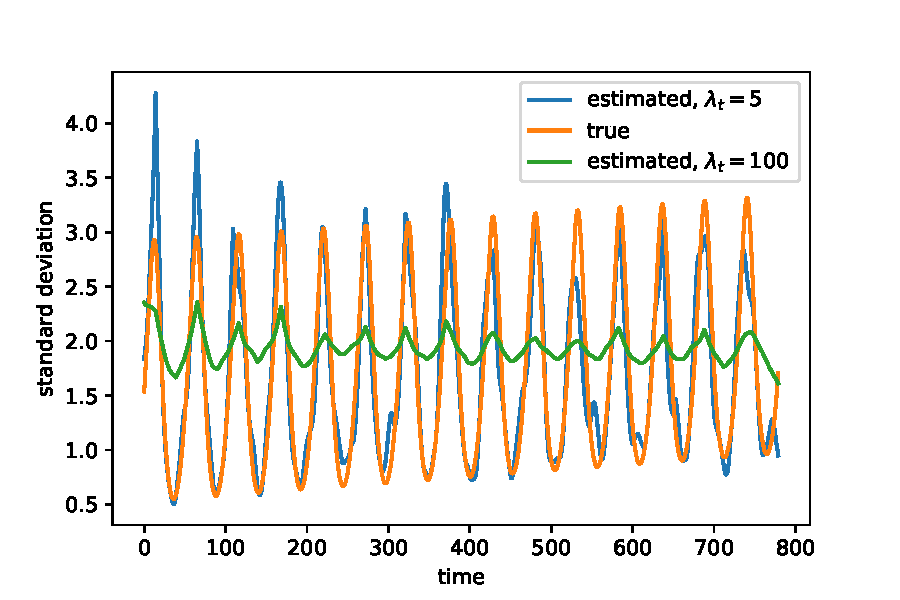
\includegraphics[height=.12\textheight]{Figures/true_fitted_var}
  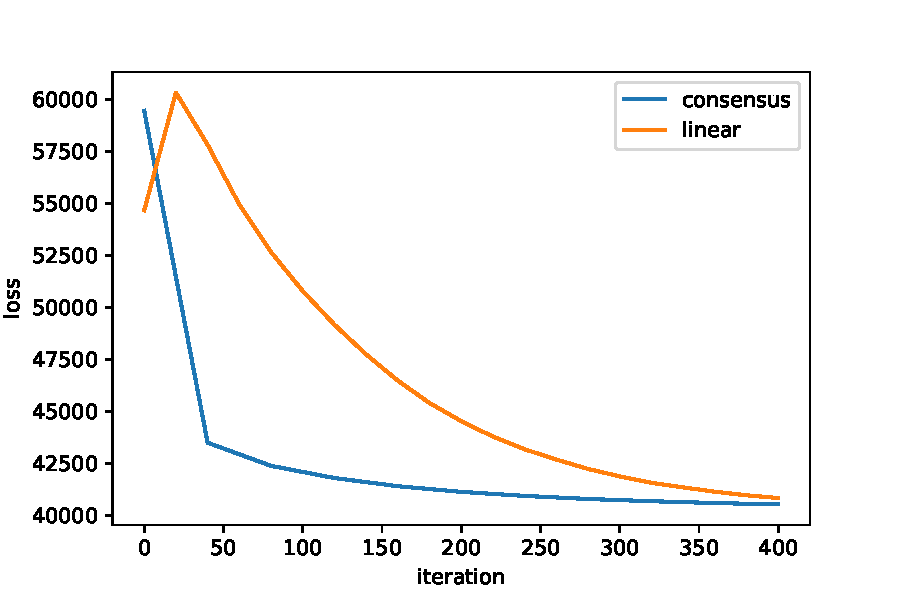
\includegraphics[height=.12\textheight]{Figures/convergence}  
  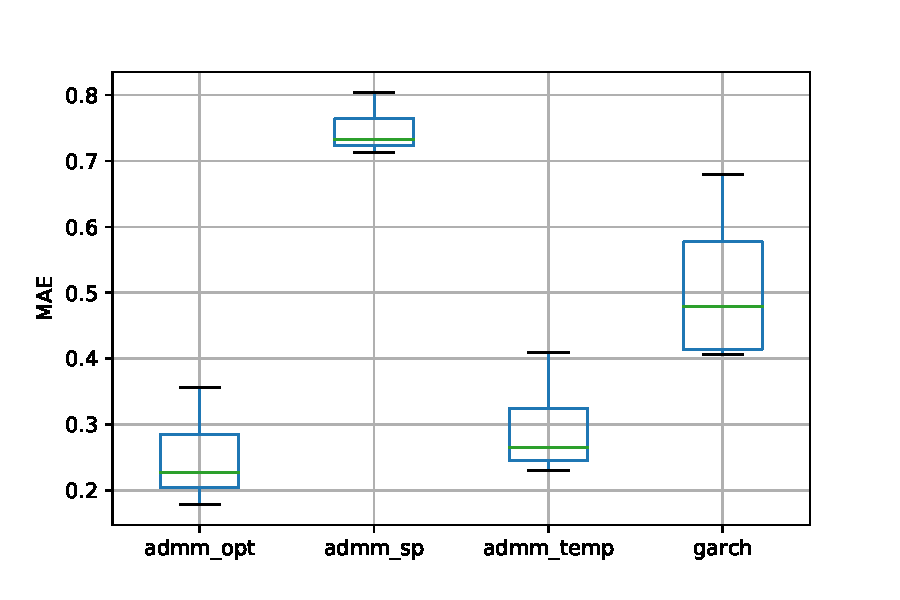
\includegraphics[height=.12\textheight]{Figures/modelComp_MAE}  
  \caption{Left: The true (orange) and estimated standard deviation 
    function at the location (0,0). The estimated values are
    obtained using linearized ADMM with $\lambda_s=0.1$ and two
    values of $\lambda_t$: $\lambda_t=5$ (blue) and
    $\lambda_t=100$ (green). Middle: Convergence speed of linearized and consensus ADMM. Right: MAE for four models: admm\_opt: the proposed model with optimal values of $\lambda_t$ and $\lambda_s$, admm\_temp: no spatial penalty, admm\_sp: no temporal penalty.} \label{fig:true_fitted_var}
\end{figure}



To further examine the performance of the proposed model, we next
compare it to three alternatives: a model which does not consider the
spatial smoothness (equivalent to fitting the model in
\autoref{sec:l1tf_var} to each time-series separately), a model which only imposes spatial smoothness, and a GARCH(1,1) model. We
simulated 100 datasets using the method explained above with $\sigma_s
\sim \mathsf{uniform}(4,7)$. The right panel of
\autoref{fig:true_fitted_var} shows the boxplot of the MAE for these
models. Interestingly, the proposed model with optimal parameters
outperforms GARCH(1,1) in estimating the true value of the variance.    


\subsection{Data analysis}
\label{sec:data}

Consensus ADMM in~\autoref{sec:consOpt} is appropriate only if
we parallelize it over multiple machines, and it is significantly
slower on our simulated data, so we do not pursue it
further here. All the results reported in this section are obtained
using \autoref{alg:linADMM}. We
applied this algorithm to the northern hemisphere of the ERA-20C
dataset available from the \href {https://www.ecmwf.int}{European Center for Medium-Range
  Weather Forecasts}. The data are
the 2 meter temperature measured daily at 12 p.m from January 1, 1960
to December 24, 2010. The Supplement explains some preprocessing and investigates some
properties of the time-series of different locations on
earth. \autoref{fig:bloom_estimatedSD} shows a processed time-series for a
single location.
The variance of this time-series has an irregular cyclic
behavior. Additionally, the time-series of other locations show 
different patterns. These observations motivated the need to develop a
non-parametric framework for this
problem. \autoref{fig:bloom_estimatedSD} also shows the
estimated SD obtained using the method of
\autoref{sec:l1tf_var}. 
% Since the estimated SD captures the periodic
% behavior of 
% volatility, it is hard to distinguish any long-term trend. Therefore,
% we compute the annual average of these 
% estimates. However, as this figure shows, the annual trend is not
% smooth. This is because in the optimization problem
% \eqref{eq:l1tf_var}, the smoothness of the annual trend is not
% encouraged. Therefore, in Appendix D we propose a simple method to
% encourage the smoothness of the annual average trend. The estimated
% SDs using this method is shown in the right panel of
% \autoref{fig:bloom_estimatedSD}. The annual average of the estimated
% SDs shows a linear trend with a positive slope.  

\paragraph{Convergence}

As shown in \autoref{alg:linADMM}, we evaluated convergence using
$\epsilon=0.001\%$ of the MSE of the data.
Our simulation experiments showed that the
convergence speed depends on the value of $\lambda_t$ and
$\lambda_s$. Furthermore, using the solution obtained for smaller values
of these parameters as a warm start for the larger values, the
converges speed improves.   


\paragraph{Model selection}
One common method for choosing the penalty parameters in the Lasso
problems is to find the solution for a range of the values of these
parameters and then choose the values which minimize a model selection
criterion. However, such analysis needs the computation of the degrees
of freedom. Several previous work have investigated the df in
generalized lasso problems
\citep{tibshirani_degrees_2012,hu_dual_2015,zeng_geometry_2017}. However,
all these studies have considered the linear regression problem and,
to the best of our knowledge, the problem of computing the df for
generalized lasso with general objective function has not been
considered yet. In this paper, we use a heuristic method for choosing $\lambda_t$ and
$\lambda_s$: we compute the optimal solution for a range of values of
these parameters and choose the values which minimize
$\mathscr{L}(\lambda_t,\lambda_s)=-l(y|h)+ \sum \lVert D_{total}h
\lVert$. This objective is a compromise between the negative log
likelihood ($-l(y|h)$) and the complexity of the solution ($\sum
\lVert D_{total}h \lVert$). For smoother solutions the value of $\sum
\lVert D_{total}h \lVert$ will be smaller but with the cost of larger
$-l(y|h)$. We computed the optimal solution for all the combinations of the
following sets of values: $\lambda_t \in \{0,2,4,8,10,15,200,1000\} \, \, ,
\lambda_s \in \{0,.1,.5,2,5,10\}$. The best combination was
$\lambda_t=4$ and $\lambda_s=2$. All the analyses in the next section
are performed on the solution for these values.  


\paragraph{Analysis of trend in temperature volatility}

\begin{figure}[tb]
  \centering
  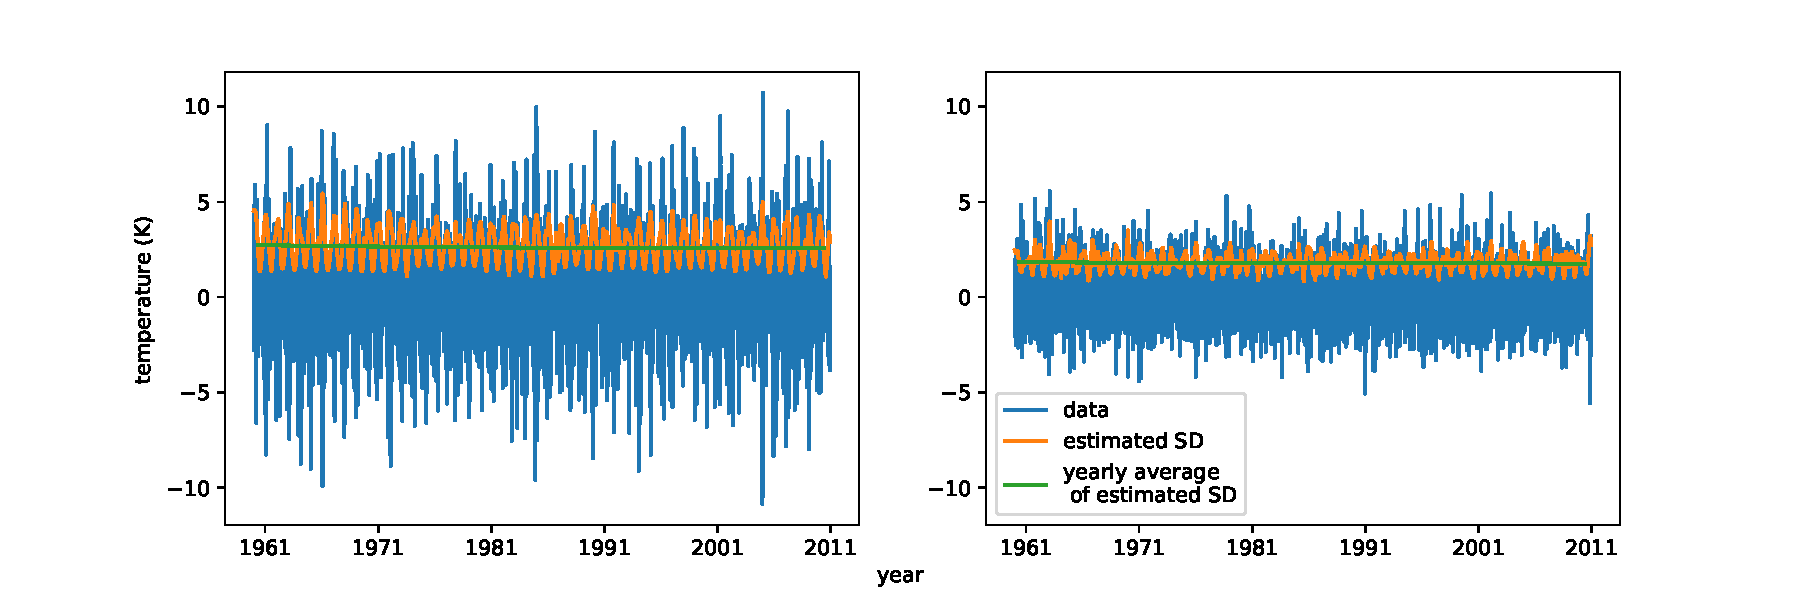
\includegraphics[width=.8 \columnwidth]{Figures/ts_estimatedVar}\\
  \caption{Detrended data and the estimated SD for
    a small midwestern city (left) and San Diego (right).} 
  \label{fig:avg_change_estimatedSD}
\end{figure} 

The top row of \autoref{fig:avg_change_estimatedSD} shows the
detrended data, the estimated standard deviation and the yearly
average of these estimates for two cities in the US: a small
midwestern city (left) and San Diego (right). The estimated SD
captures the periodic behavior in the variance of the time-series. In
addition, the number of linear segments changes adaptively in each
time window depending on how fast the variance is changing.  
\begin{figure}[tb]
  \centering
  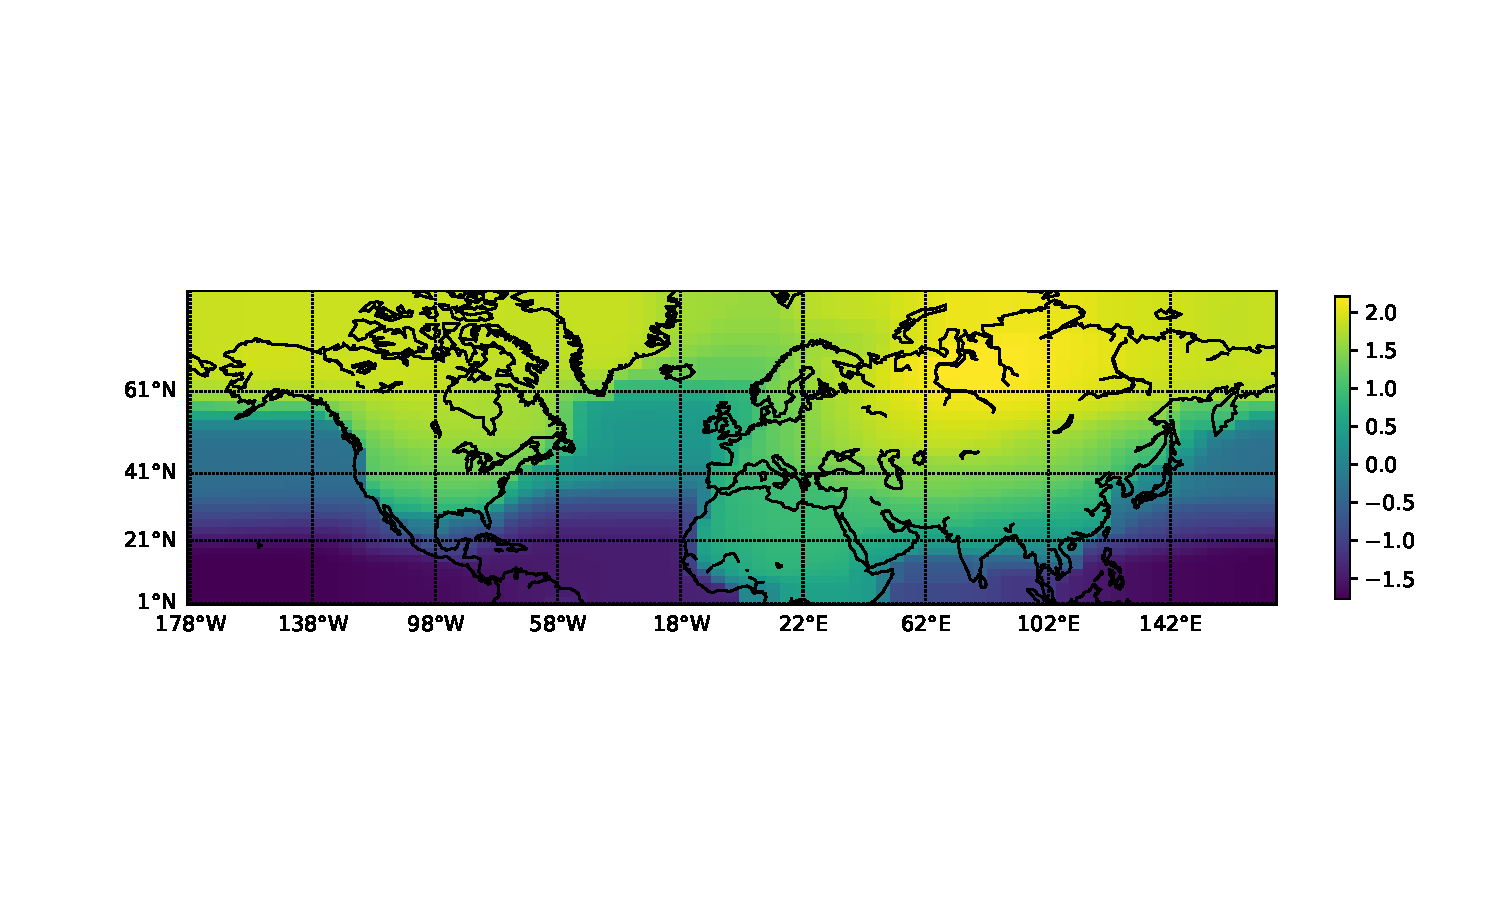
\includegraphics[width=.45\linewidth]{Figures/avg_logVar.pdf}
  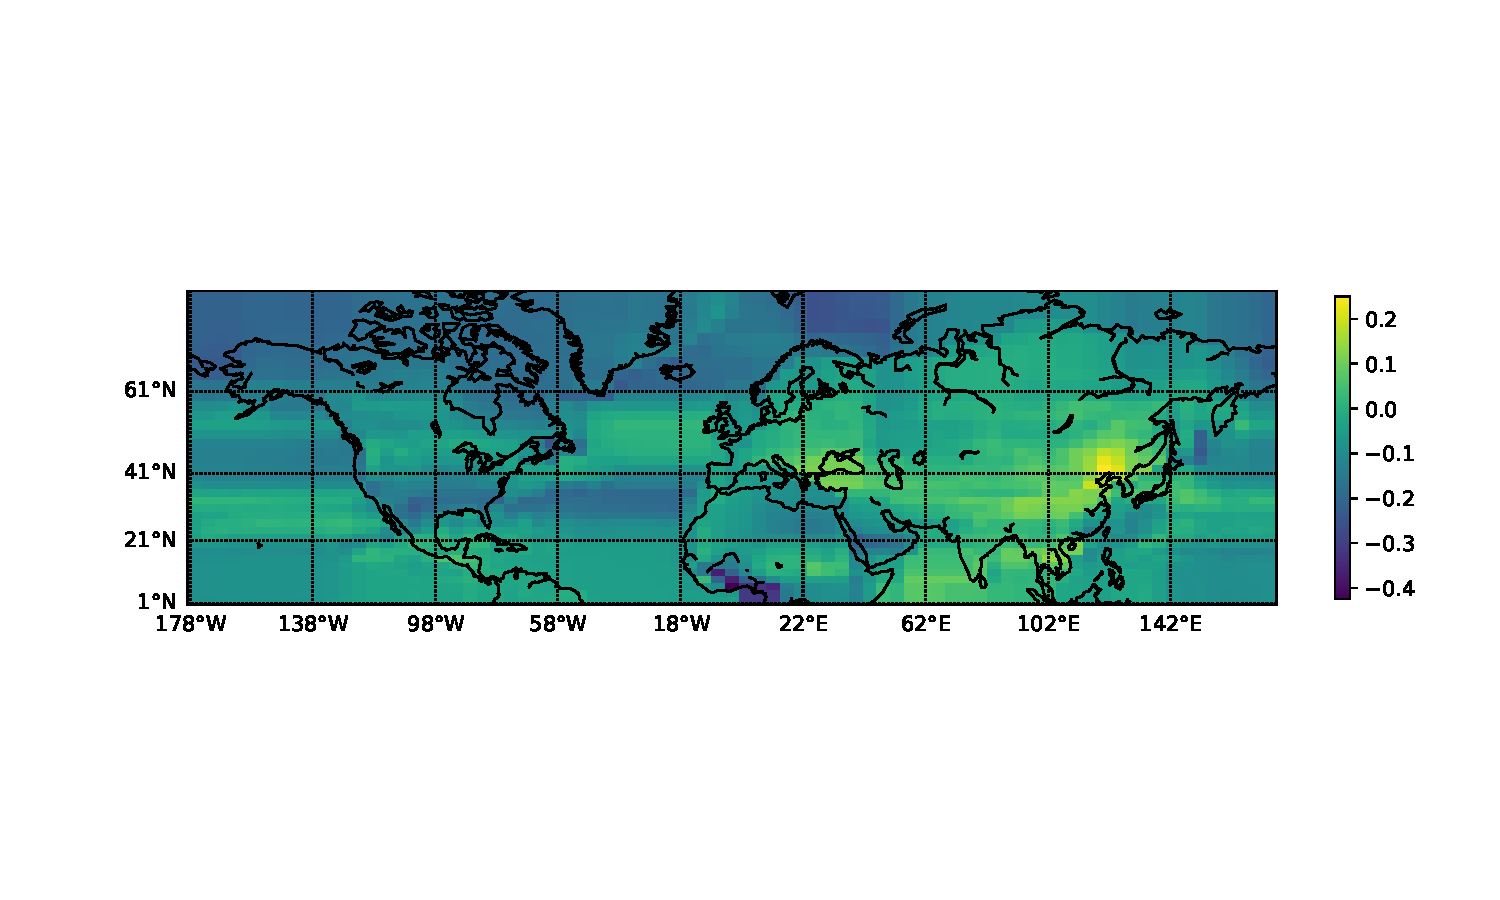
\includegraphics[width=.45\linewidth]{Figures/avg_change_logVar.pdf}
  \caption{The
    average of the estimated variance over the northern hemisphere (left) and the
    change in the variance from 1961 to 2011 (right).}
\label{fig:avg_chg}
\end{figure}

The yearly average of the estimated SD captures the trend in the
temperature volatility. For example, we can see that the variance in
the midwestern city displays a small positive trend. To determine how the volatility has
changed in each location, we subtract the average of the estimated
variance in 1961 from the average in the following years and compute
their sum. The value of this change in the variance in each location
is depicted in the right panel of
\autoref{fig:avg_chg}. The left panel of this
shows the average estimated variance in each location. Since the
optimal value of the spatial penalty is rather large ($\lambda_s=2$)
the estimated variance is spatially very smooth. 

It is interesting to note that the trend in volatility is almost zero
over the oceans. The most positive trend can be observed in Asia and
particularly in south-east Asia. 

\begin{figure}[tb]
  \centering
  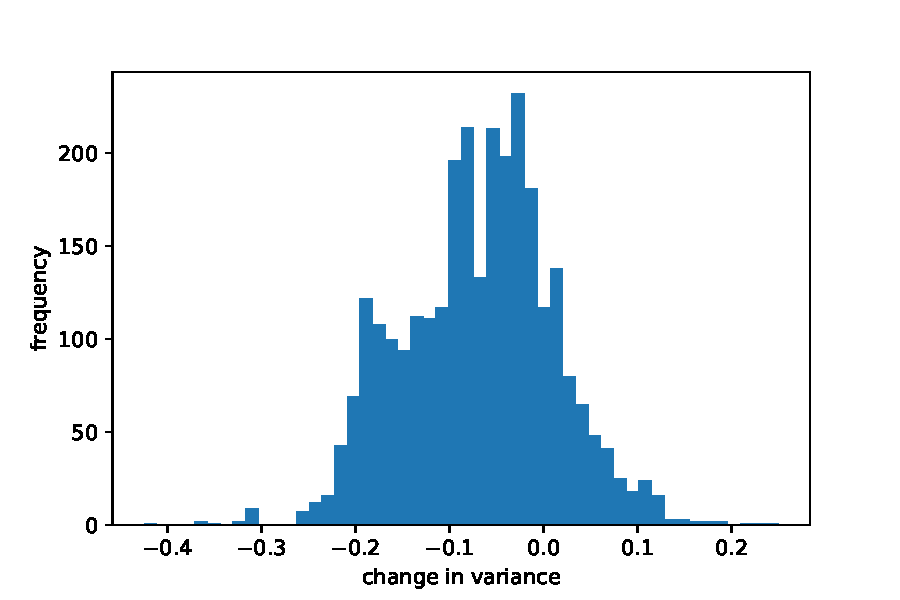
\includegraphics[width=.3\linewidth]{Figures/hist_avg_change.pdf}
  \caption{The histogram of changes in estimated SD.}
  \label{fig:hist}
\end{figure}

\autoref{fig:hist} shows the
histogram of change in the estimated SD across the northern
hemisphere. The SD in most locations on the northern
hemisphere had a negative trend in this time period, though spatially,
this decreasing pattern is localized mainly toward the extreme
northern latitudes and over oceans. In many ways, this is consistent
with climate change predictions: oceans tend to operate as a local
thermostat, regulating deviations in local temperature, while warming polar
regions display fewer days of extreme cold.



 

\section{Discussion}
In this paper, we proposed a new method for estimating the variance of
spatio-temporal data. The main idea is to cast this problem as a
constrained optimization problem where the constraints enforce smooth
changes in the variance for neighboring points in time and space. In
particular, the solution is piecewise linear in time and piecewise
constant in space. The resulting optimization is in the form of a
generalized LASSO problem with high-dimension, and so applying the
PDIP method directly is infeasible. We therefore developed two
ADMM-based algorithms to solve this problem: the consensus ADMM and
linearized ADMM. 

The consensus ADMM algorithm converges in a few hundreds of iterations
but each iteration takes much longer than the linearized ADMM
algorithm. The appealing feature of the consensus ADMM algorithm is
that if it is parallelized on enough machines the
computation time per iteration remains constant as the problem size
increases. The linearized ADMM algorithm on the other hand converges
in a few thousand iterations but each iteration is performed in a
split second. However, since the algorithm converges in many
iterations it is not very appropriate for parallelization. The reason
is that after each iteration the solution computed in each machine
should be broadcast to the master machine and this operation takes
some time which depends on the speed of the network connecting the
slave machines to the master. A direction for future research would be
to combine these two algorithms in the following way: the problem
should be split into the sub-problems (as in the consensus ADMM) but
each sub-problem can be solved using linearized ADMM. 

% \attn{We did not do this. Change the below.}
% We applied the linearized ADMM algorithm to the surface temperature
% data on a grid over the united states, for years 1992-2002. The
% results showed that in many locations the variance of the temperature
% has increased about 1 unit in 10 years. 

% The goal of this paper, however, is not to make any conclusions about
% the trend in the variance because we solved the problem only for a
% grid over the united states and for 10 years of the data. A thorough
% analysis, needs the full solution over the globe and for a longer time
% period. The goal of the paper, was to propose the idea of estimating
% the trend in variance of spatio-temporal signals using generalized
% lasso and to investigate the algorithms for solving the resulting
% optimization problem. 


 
\newpage
\bibliographystyle{abbrvnat}
\small
\bibliography{nips-references}


\end{document} 

